Modern computing devices are becoming ever smaller, and to do this they must be engineered to combat the ever encroaching quantum effects at these scales, with increasing difficulty. Intel's current process incorporates a 14nm FET channel, as such the design of these FETs has been greatly changed to eliminate quantum effects.\cite{intel_process}

The trend in transistor miniaturisation has been dubbed "Moore's Law", following a prediction made by Gordon Moore, co-founder of Intel, in 1965.\cite{moores_law} Despite the remarkable accuracy of his prediction, many predict \cite{end_of_Moore_1, end_of_Moore_2} the inevitable breakdown as the physical limitations of creating such devices exponentially increases the start-up cost of manufacturing, as well as cost of research and development.

\begin{figure}[htbp!]
	\centering
	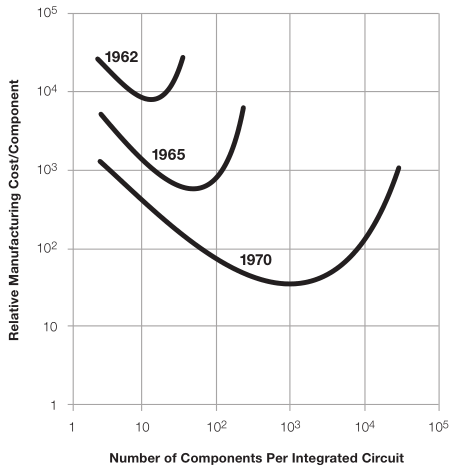
\includegraphics[width=0.8\textwidth]{moores_law}
	\caption{Gordon Moore's Prediction on Component Cost - Moore's Law}
	\label{fig::moores_law}
\end{figure}
